\documentclass[journal,12pt,twocolumn]{IEEEtran}

\usepackage{tikz}
\usepackage{setspace}
\usepackage{gensymb}
\singlespacing

\usepackage{amsmath}
\usepackage{amsthm}
\usepackage{txfonts}
\usepackage{cite}
\usepackage{enumitem}
\usepackage{mathtools}
\usepackage{listings}
    \usepackage{color}                                            
    \usepackage{array}                                            
    \usepackage{longtable}                                        
    \usepackage{calc}                                             
    \usepackage{multirow}                                         
    \usepackage{hhline}                                           
    \usepackage{ifthen}                                           
 
    \usepackage{lscape}     
\usepackage{multicol}
\usepackage{chngcntr}
\renewcommand\thesection{\arabic{section}}
\renewcommand\thesubsection{\thesection.\arabic{subsection}}
\renewcommand\thesubsubsection{\thesubsection.\arabic{subsubsection}}

\renewcommand\thesectiondis{\arabic{section}}
\renewcommand\thesubsectiondis{\thesectiondis.\arabic{subsection}}
\renewcommand\thesubsubsectiondis{\thesubsectiondis.\arabic{subsubsection}}

% correct bad hyphenation here
\hyphenation{op-tical net-works semi-conduc-tor}
\def\inputGnumericTable{}                                 %%

\lstset{
%language=C,
frame=single, 
breaklines=true,
columns=fullflexible
}
\begin{document}
\title{Assignment No.1}
\author{Akash Subhash Kamble (sm21mtech11002)}
\maketitle

\section{chapter2,Problem No:14.2}
Problem Statement:Find the in-centres of the triangles whose vertices are as follows,
(5,3), (5,-1), (-7,-6)\\

\textbf{Solution}\\

Given: A(5,3) ,B(5,-1), C(-7,-6)\\

To find in-centre now calculate unit length of each side of a triangle\\
Here 
\begin{align*}
x_1&=5 & y_1&=3\\
x_2&=5 & y_2&=-1\\
x_3&=-7 & y_3&=-6
\end{align*}
\begin{align*}
BC=a&=\sqrt{(x_3-x_2)^2+(y_3-y_2)^2}\\
&=\sqrt{-12^2+5^2}\\
&=13    
\end{align*}
Similarly,
\begin{align*}
CA=b&=15\\
AB=c&=4
\end{align*}

Now find in-centre of a triangle,\\
\begin{align*}
In-centre&=(\frac{ax_1+bx_2+cx_3}{a+b+c},\frac{ay_1+by_2+cy_3}{a+b+c})\\
&=(\frac{65+75-28}{32},\frac{39-15-24}{32})\\
&=(3.5,0)
\end{align*}

\begin{figure}[!ht]
	\centering
	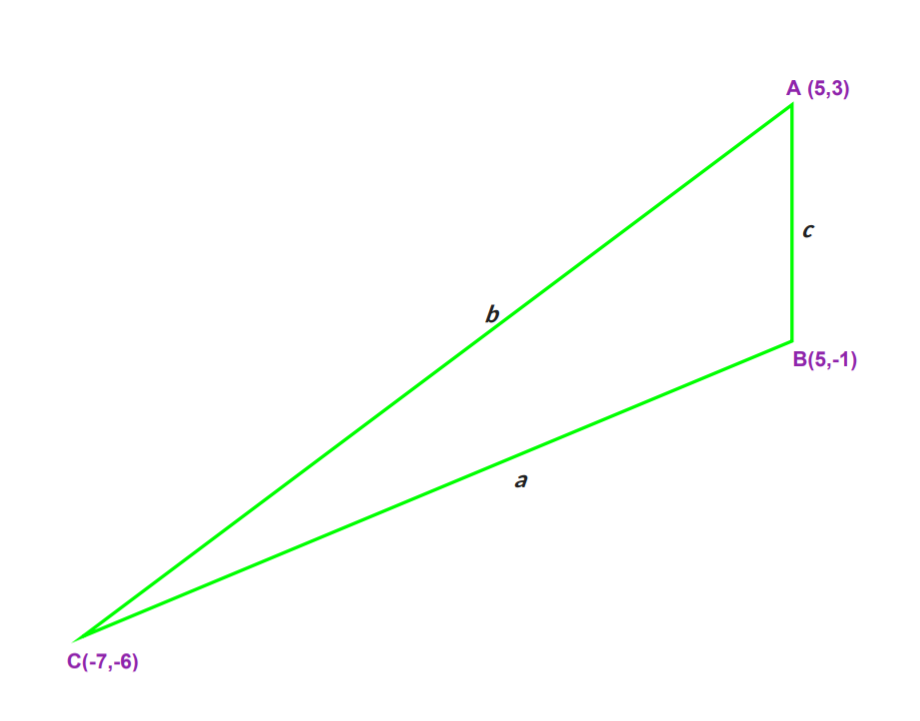
\includegraphics[width=\columnwidth]{tri.png}
	\caption{A Triangle for given points}

\end{figure}


\end{document}